\documentclass[11pt,                    % corpo del font principale
               a4paper,                 % carta A4
               %twoside,                 % impagina per fronte-retro
               %openright,               % inizio capitoli a destra
               english,
               %italian,
               ]{article}

%**************************************************************
% Importazione package
%**************************************************************

\usepackage{amsmath,amssymb,amsthm}    % matematica
%\usepackage[english, italian]{babel}    % per scrivere in italiano e in inglese;
\usepackage[english]{babel}    % per scrivere in italiano e in inglese;
                                        % l'ultima lingua (l'italiano) risulta predefinita
\usepackage[top=1.5in,bottom=1in,right=1in,left=1in,headheight=65pt,headsep=1cm]{geometry}
%\usepackage[paperwidth=5.5in, paperheight=8.5in]{geometry}


\usepackage{float}

\usepackage{caption}                    % didascalie

\usepackage{chngpage,calc}              % centra il frontespizio

\usepackage{csquotes}                   % gestisce automaticamente i caratteri (")

\usepackage{emptypage}                  % pagine vuote senza testatina e piede di pagina

\usepackage{epigraph}                   % per epigrafi
\usepackage[bottom]{footmisc}           % put footnotes at the bottom
\usepackage{eurosym}                    % simbolo dell'euro
\usepackage{enumitem}        % separation between list items
\usepackage{ifxetex}                    %compilazione xelatex

\ifxetex

\RequirePackage{xltxtra,fontspec,xunicode}

\RequirePackage{unicode-math}

\else
  \RequirePackage[utf8]{inputenc}

\fi


\usepackage{verbatim}

\usepackage{graphicx}                   % immagini

\usepackage[
    colorlinks=true,       % false: boxed links; true: colored links
    linkcolor=cyan,          % color of internal links (change box color with linkbordercolor)
    citecolor=cyan,        % color of links to bibliography
    filecolor=magenta,      % color of file links
    urlcolor=cyan,          % color of external links
]{hyperref}                   % collegamenti ipertestuali


\usepackage{longtable} % per le tabelle multipagina
\usepackage{listings}                   % codici

\usepackage{microtype}                  % microtipografia

\usepackage{mparhack,fixltx2e,relsize}  % finezze tipografiche

\usepackage{nameref}                    % visualizza nome dei riferimenti

\usepackage[font=small]{quoting}        % citazioni

\usepackage{subcaption}                     % sottofigure, sottotabelle

\usepackage[section]{placeins} %\FloatBarrier

\usepackage[italian]{varioref}          % riferimenti completi della pagina

\usepackage[dvipsnames]{xcolor}         % colori

\usepackage{booktabs}                   % tabelle
\usepackage{tabularx}                   % tabelle di larghezza prefissata
\usepackage{longtable}                  % tabelle su più pagine
\usepackage{indentfirst}
\usepackage{ltxtable}                   % tabelle su più pagine e adattabili in larghezza
\usepackage[toc, acronym]{glossaries}   % glossario
                                        % per includerlo nel documento bisogna:
                                        % 1. compilare una prima volta tesi.tex;
                                        % 2. eseguire: makeindex -s tesi.ist -t tesi.glg -o tesi.gls tesi.glo
                                        % 3. eseguire: makeindex -s tesi.ist -t tesi.alg -o tesi.acr tesi.acn
                                        % 4. compilare due volte tesi.tex.

\usepackage[backend=bibtex,style=ieee,hyperref,backref]{biblatex}
                                        % eccellente pacchetto per la bibliografia;
                                        % produce uno stile di citazione autore-anno;
                                        % lo stile "numeric-comp" produce riferimenti numerici
                                        % per includerlo nel documento bisogna:
                                        % 1. compilare una prima volta tesi.tex;
                                        % 2. eseguire: biber tesi
                                        % 3. compilare ancora tesi.tex.


\usepackage[linesnumbered,ruled,vlined]{algorithm2e}% Use the algorithmicx package for pseudocode
%\usepackage{algorithm}
%\usepackage{algpseudocode}

%verbatim
\usepackage{fancyvrb}

%\usepackage{fancyhdr}
%\pagestyle{fancy}

%\rfoot{Pagina: \emph{ \thepage\ / \pageref{LastPage}}}


\title{Report Assignment 1 - Large Scale Data Engineering}


% Place the author information here.  Please hand-code the contact
% information and notecalls; do *not* use \footnote commands.  Let the
% author contact information appear immediately below the author names
% as shown.  We would also prefer that you don't change the type-size
% settings shown here.

\author{
Alberto Simioni, 2577392 \\
Federico Ziliotto, 2577394
}\date{\today}


%********        Headers e footer       ***********************%

%\fancyhead[R]{\small\rightmark}
%\fancyhead[L]{\small\leftmark}
%\fancyfoot[C]{\small\thepage}
%\fancyhead[LO]{\small\leftmark}% odd page header and number to right top
%\fancyhead[RE]{\small\leftmark}%Even page header and number at left top
%\fancyfoot[L,R,C]{}
%\renewcommand{\headrulewidth}{0pt}% disable the underline of the header part


% \lhead{\textsc{\title}}
% \chead{}
% \rhead{\rightmark}
% %\lfoot{\thepage}
% \cfoot{\thepage}
% %\rfoot{\textsc{\leftmark}}


%line spacing
\linespread{1.2}
\setlist{nosep}
\setlength{\parindent}{14pt}   % larghezza rientro della prima riga
%\setlength{\parskip}{10pt}   % distanza tra i paragrafi


%%--------------------------------------------------------------------------
%% Font settings
%%--------------------------------------------------------------------------
\ifxetex
\setromanfont{Adobe Text Pro}
\setsansfont{Myriad Pro}
%\setmonofont{Source Code Pro}

% Microsoft set
% \setromanfont{Cambria}
% \setsansfont{Calibri}
 \setmonofont{Consolas}
\setmathfont{Cambria Math}
\else
  \usepackage[T1]{fontenc}
  \usepackage{newtxtext,newtxmath}
%Font packages
%\usepackage{times}
 %\usepackage{lmodern}
 %\usepackage{mathpazo}
 %\usepackage{kpfonts}
 %\usepackage{mathptmx}
 %\usepackage{times,mtpro2}
 %\usepackage{stix}
 %\usepackage{txfonts}
 %\usepackage{newtxtext,newtxmath}
 %\usepackage{libertine} \usepackage[libertine]{newtxmath}
%\usepackage{newtxtext,newtxmath}
\fi


%%--------------------------------------------------------------------------
%% Algorithms settings
%%--------------------------------------------------------------------------
\newcommand\mycommfont[1]{\scriptsize\ttfamily\textcolor{blue}{#1}}
\SetCommentSty{mycommfont}

\makeatletter
\renewcommand{\listalgorithmcfname}{Lista degli Algoritmi}%
\renewcommand{\algorithmcfname}{Algoritmo}%
\renewcommand{\algocf@typo}{}%
\renewcommand{\@algocf@procname}{Procedura}
\renewcommand{\@algocf@funcname}{Funzione}
\makeatother

\floatstyle{ruled}
\newfloat{program}{thbp}{lop}
\floatname{program}{Programma}

\floatstyle{ruled}
\newfloat{algorithm}{thb}{lop}
\floatname{algorithm}{Algoritmo}


%**********   Hyperlink setup ************%
\hypersetup{
    bookmarks=true,         % show bookmarks bar?
    pdftoolbar=true,        % show Acrobat’s toolbar?
    pdfmenubar=true,        % show Acrobat’s menu?
    pdffitwindow=false,     % window fit to page when opened
    pdfstartview={FitH},    % fits the width of the page to the window
    pdftitle={},    % title
    pdfauthor={},     % author
    pdfsubject={},   % subject of the document
    %pdfcreator={Federico Ziliotto},   % creator of the document
    %pdfproducer={Producer}, % producer of the document
    pdfkeywords={}, % list of keywords
    pdfnewwindow=true,      % links in new PDF window
    colorlinks=true,       % false: boxed links; true: colored links
    linkcolor=cyan,          % color of internal links (change box color with linkbordercolor)
    citecolor=cyan,        % color of links to bibliography
    filecolor=magenta,      % color of file links
    urlcolor=cyan           % color of external links
}
%**************************************************************
% Impostazioni di caption
%**************************************************************
\captionsetup{
    tableposition=top,
    figureposition=bottom,
    font=small,
    format=hang,
    labelfont=bf
}



%**************************************************************
% Impostazioni di glossaries
%**************************************************************
%\input{glossario} % database di termini
\makeglossaries


%**************************************************************
% Impostazioni di graphicx
%**************************************************************
\graphicspath{{Images/}} % cartella dove sono riposte le immagini


%**************************************************************
% Impostazioni di itemize
%**************************************************************
%\renewcommand{\labelitemi}{$\ast$}

\renewcommand{\labelitemi}{$\bullet$}
%\renewcommand{\labelitemii}{$\cdot$}
%\renewcommand{\labelitemiii}{$\diamond$}
%\renewcommand{\labelitemiv}{$\ast$}


%**************************************************************
% Impostazioni di listings
%**************************************************************
\lstset{
    language=[LaTeX]Tex,%C++,
    keywordstyle=\color{RoyalBlue}, %\bfseries,
    basicstyle=\small\ttfamily,
    %identifierstyle=\color{NavyBlue},
    commentstyle=\color{Green}\ttfamily,
    stringstyle=\rmfamily,
    numbers=none, %left,%
    numberstyle=\scriptsize, %\tiny
    stepnumber=5,
    numbersep=8pt,
    showstringspaces=false,
    breaklines=true,
    frameround=ftff,
    frame=single
}


%**************************************************************
% Impostazioni di biblatex
%**************************************************************
%\bibliographystyle{unsrtnat}

\bibliography{bibliography} % database di biblatex
%\bibliographystyle{alpha}
%\addbibresource{bibliography.bib}




%\author
%{John Smith,$^{1\ast}$ Jane Doe,$^{1}$ Joe Scientist$^{2}$\\
%\\
%\normalsize{$^{1}$Department of Chemistry, University of Wherever,}\\
%\normalsize{An Unknown Address, Wherever, ST 00000, USA}\\
%\normalsize{$^{2}$Another Unknown Address, Palookaville, ST 99999, USA}\\
%\\
%\normalsize{$^\ast$To whom correspondence should be addressed; E-mail:  jsmith@wherever.edu.}
%}



%%%%%%%%%%%%%%%%% END OF PREAMBLE %%%%%%%%%%%%%%%%



% Double-space the manuscript.


% Make the title.



\begin{document}
\maketitle

%\include{Sections/Introduzione.tex}
%\include{Section2}
%\include{Section3}
%\include{Section4}
%\include{Conclusion}

%*******    Figure and Subfigure example ***********
%\begin{figure}[tbh]
% \includegraphics[width=1\linewidth]{circle}
% \caption[Circonferenza]{Circle}
% \label{fig:circle}
% \end{figure}%

% \begin{figure}[tbh]
% \begin{subfigure}{.5\textwidth}
% \includegraphics[width=1\linewidth]{circle}
% \caption[Circonferenza]{Circle}
% \label{fig:circle}
% \end{subfigure}%
% \begin{subfigure}{0.5\textwidth}
% \includegraphics[width=1\linewidth]{random}
% \caption[Random]{Random}
% \label{fig:random}
% \end{subfigure}
% \end{figure}
%%%***************************************%%



% Place your abstract within the special {sciabstract} environment.




% In setting up this template for *Science* papers, we've used both
% the \section* command and the \paragraph* command for topical
% divisions.  Which you use will of course depend on the type of paper
% you're writing.  Review Articles tend to have displayed headings, for
% which \section* is more appropriate; Research Articles, when they have
% formal topical divisions at all, tend to signal them with bold text
% that runs into the paragraph, for which \paragraph* is the right
% choice.  Either way, use the asterisk (*) modifier, as shown, to
% suppress numbering.

\section{Data Size Analysis}
The main bottleneck of the basic algorithm is memory. With only 1GB of available memory and binary files to load for a total of ~5.6GB (\texttt{person, interest and knows maps}) we first analyzed the query to look for ways to drop unnecessary data. The possible optimization we found were:
\begin{enumerate}
    \item Consider only relationships between people in the same location: the query searches for friendships of people that live in the same city, while the \texttt{knows} file contains all relationships. By removing those between people in different cities we both reduce the size of the data we have to look into and the computation cost of searching through friendships that are not important for the results of the query;
    \item Consider only mutual friendships: each person can have a knows relationship with each other but this is unilateral. Since the query asks for only mutual relationships between two person (if P1,P2 are two persons, then in the \texttt{knows map} we can find both P1->P2 and P2->P1) we drop all single relationships between people;
    \item Remove people that don't have any mutual friendship with someone in the same city: it follows directly from the steps above, these type of people are not useful because they will surely not be result of the query.
\end{enumerate}
After applying these optimizations we created the files:
\begin{itemize}
    \item \texttt{knows\_location}: original knows that contains only relationships between people in the same location;
    \item \texttt{person\_location}: person map with updated indexes knows\_first and knows\_n to reflect the knows\_location;
    \item \texttt{knows\_mutual}: knows relationships only between people that know each other;
    \item \texttt{person\_mutual}: person map that contains only people that have at least a mutual friendship in the same location and has the correct indexes knows\_first and knows\_n (for the knows\_mutual);
\end{itemize}


\section{Interests inverted table}


\section{Birthday ordering}
In the naive implementation we run through the entire \texttt{person\_map} and check every time if the current person has the birthday in the range of the query. We decided to optimize the access to the data by ordering the person by birthday. We had two options: order the people in the data structure (and update the indexes contained in the interests and knows files) or create a new index containing the position of the person and its birthday and then order it. We decided to go for the latter that was easier to implement without modifying the other data structures but has the disadvantage that it uses more memory. \\
In the cruncher, we use the birthday index to first search the first occurrence of a person with a birthday in the range required by the current query, then we know all the people inside the range follows the first one until we reach someone with a birthday that is out of the bound.

\section{Data Structures}

\begin{figure}[tbh]
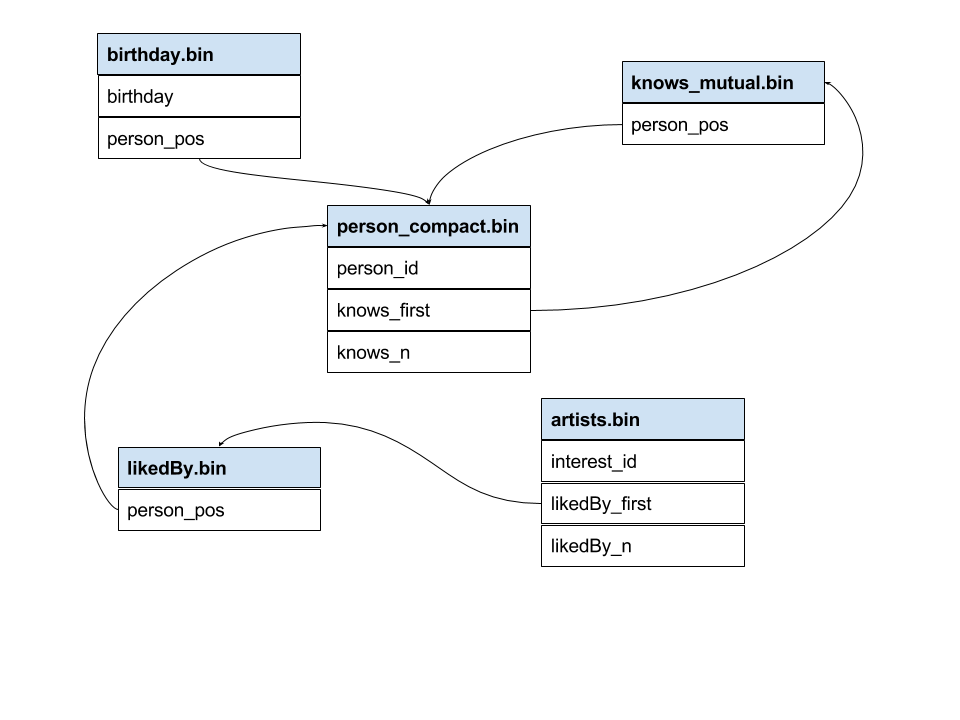
\includegraphics[width=1\linewidth]{data}
\caption[Data]{Data}
\label{fig:data}
\end{figure}

In figure \ref{fig:data} we show the data structure used by the cruncher to perform the queries. The intermediate files created are not shown in the figure. Since we use a different table for the people's birthdays and the interests table now has a reference to the person's one, we decided to drop the birthday, interest\_first and interest\_n fields from the Person data type to reduce even more the total size.


\section{Cruncher}

\section{Possible improvements}
\begin{itemize}
    \item To save the relationships between people we use a person table that contains all the people and a knows table that has the offsets to the person table. Another way to obtain the same result would be to use a unified table of couples with two person\_id for each entry. This would improve the sequential access to the data (the id of two person who are friend are always close to each other) 
    \item Instead of using a secondary file to index the birthdays we could have ordered the people in the data structures to reduce the memory usage;
    \item For each query, we load the \texttt{artists} and \texttt{likedBy} files to calculate the scores for the query in questions. We could calculate the scores for all the queries (or for a bunch of them) at a time and store them in an array (the number of queries should be small enough to avoid occupying too much memory with this array) so that we wouldn't need to access those files frequently;
    \item An alternative to the a\texttt{artists} and \texttt{likedBy} files we use would be to create a bit array of size \texttt{number\_of\_person * number\_of\_interests} where each bit set to 1 if a person likes an artist. In a scenario where the amount of 1s is around half of the total (each person on average likes half of the artists) this would be a good way to compact the data. In this case we found that each person likes only a few of the artists available, so implementing the bit array would have led to a structure filled with mostly 0s. 
\end{itemize}





\clearpage

%\bibbycategory % equivale a dare un \printbibliography per ogni categoria

\end{document}
